\part{Arithmetik und Algebra I}\index{Arithmetik und Algebra!I|textbf}
\renewcommand{\bbwPartID}{AA1}
%%
%% 2019 07 04 Ph. G. Freimann
%%

\section{Zahlen}
\sectuntertitel{Im 15. Jahrhundert --- genauer im Jahre 1413 --- am
  zwölften elften um zehn Uhr neun haben acht der sieben Schlauesten
  gesagt: ``So sechs wie wir fünf gibt's keine vier mehr, denn wir
  drei sind die zwei einzigen Nullen.``}



%%\TALSTadBFWA{8}{1.1}
%%%%%%%%%%%%%%%%%%%%%%%%%%%%%%%%%%%%%%%%%%%%%%%%%%%%%%%%%%%%%%%%%%%%%%%%%%%%%%%%%
\subsection*{Lernziele}

\begin{itemize}
	\item Zahlmengen $\mathbb{N}$, $\mathbb{Z}$, $\mathbb{Q}$, $\mathbb{R}$
  \item Näherungswerte, Runden
  \item Wissenschaftliche Notation
  \item Ordnungsrelationen ($=$, $<$, $>$, $\leq$, $\geq$)
  \item Betrag
\end{itemize}

\TadBMTA{13}{1.1}

\newpage

\subsection{Die natürlichen Zahlen ($\mathbb{N}$)}\index{Zahlen!natürliche}

\begin{definition}{natürliche Zahlen}{definition_natuerliche_zahlen}
  Natürliche Zahlen $\mathbb{N}$ sind ganze positive Zahlen: ${1, 2, 3, 4, 5, ....}$.
\end{definition}

\TALS{
  \begin{bemerkung}{Null}{}
  Selten wird auch die Menge ${0, 1, 2, 3, 4, ...}$ als die Menge
  der natürlichen Zahlen bezeichnet. Wenn die Unterscheidung
  wesentlich ist, verzichten wir auf die Schreibweise $\mathbb{N}$ und
  verwenden

  $$\mathbb{N}_0 = \mathbb{N}\cup{} \{0 \}  = \{0, 1, 2, 3, 4, ...\}$$
  bzw.
  $$\mathbb{N}\backslash\{0\} =\mathbb{N}^\ast= \mathbb{N}^+= \{1, 2, 3, 4, ...\}.$$
  \end{bemerkung}
}%% END TALS

\GESO{\begin{bemerkung}{Notation}{}
  Um explizit anzugeben, dass die Zahl Null nicht zu $\mathbb{N}$ gehört schreiben wir:
  $$\mathbb{N}\backslash{}\{0\}$$
  Um explizit anzugeben, dass die Zahl Null zur Menge $\mathbb{N}$ gehören soll, schreiben wir:
  $$\mathbb{N}_0$$
\end{bemerkung}}%% END GESO


Mit natürlichen Zahlen können wir beliebig
\begin{itemize}
\item \LoesungsRaumLang{\textbf{addieren} ($+$)}  und
\item \LoesungsRaumLang{\textbf{multiplizieren} ($\cdot{}$)}.
\end{itemize}

\begin{bemerkung}{Subtraktion}{}
  Eine Subtraktion ist in den natürlichen Zahlen nur bedingt möglich:
  \TNT{4}{
  $$8-4 \in \mathbb{N}$$
  aber:
  $$3-6 \not\in \mathbb{N}$$}%% END TNT
\end{bemerkung}
\newpage


\subsection{Ganze Zahlen ($\mathbb{Z}$)}\index{Zahlen!ganze}
\begin{definition}{ganze Zahlen}{definition_ganze_zahlen}

  Mit $\mathbb{Z}$ bezeichnen wir alle ganzen Zahlen, sowohl die
  positiven ($\mathbb{N}$), wie auch die negativen.
  \end{definition}

$$\mathbb{Z} = \{..., -3, -2, -1, 0, 1, 2, 3,  4, ... \}$$

Mit den ganzen Zahlen sind uneingeschränkt durchführbar:
\begin{itemize}
\item Addition ($+$)
  \item Multiplikation ($\cdot$)
\item \LoesungsRaumLang{\textbf{Subtraktion} ($-$)}
  \end{itemize}


\begin{bemerkung}{Division}{}
  Eine Division ist in den ganzen Zahlen nur bedingt möglich:
  \TNT{3.6}{
  $$8:4 \in \mathbb{Z}$$
  aber:
  $$5:3 \not\in \mathbb{Z}$$}%% END TNT
\end{bemerkung}


\TALS{
\subsubsection{Zahlenstrahl / Zahlengerade}\index{Zahlenstrahl}

\begin{center}
\raisebox{-1cm}{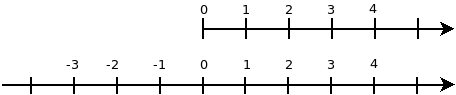
\includegraphics[width=13cm]{allg/alg/img/Zahlenstrahl.png}}
\end{center}

Der Zahlenstrahl hat den Startpunkt 0 (Null)\footnote{... manchmal  den Startpunkt 1 ...}, wohingegen die
Zahlengerade auf beiden Seiten uneingeschränkt weiterläuft.%%
}%% END TALS

\newpage


\subsection{Rationale Zahlen ($\mathbb{Q}$)}
\index{Zahlen!rationale}\index{rationale Zahlen}

\begin{definition}{rationale Zahlen}{}
Zahlen, welche sich als Bruch mit ganzen Zahlen schreiben lassen,
werden als \textbf{rationale Zahlen} bezeichnet.


$$\mathbb{Q} =\left\{ q = \frac{a}{b} \,\,\, \middle| \,\,\, a,b \in
\mathbb{Z}, b \ne 0 \right\}$$
\end{definition}

\subsubsection{Beispiele}

$$0.5 = \LoesungsRaum{\frac12} \hspace{1cm} (a=\LoesungsRaum{1}; b=\LoesungsRaum{2})$$

$$3 = \LoesungsRaum{\frac31} \hspace{1cm} (a=\LoesungsRaum{3}; b=\LoesungsRaum{1})$$

oder so:

$$-8 = \LoesungsRaum{\frac{-16}{2}} \hspace{1cm} (a=\LoesungsRaum{-16}; b=\LoesungsRaum{2})$$

$$0 = \LoesungsRaum{\frac{0}{7}} \hspace{1cm} (a=\LoesungsRaum{0}; b=\LoesungsRaum{7})$$


Mit den \textbf{rationalen} Zahlen sind uneingeschränkt durchführbar:
\begin{itemize}
\item Addition ($+$)
  \item Multiplikation ($\cdot$)
\item Subtraktion ($-$)
\item \LoesungsRaumLang{\textbf{Division} ($:$
  bzw. $\frac{\cdot{}}{\cdot{}}$ bzw. $\frac{\Box{}}{\Box{}}$)}
  \end{itemize}

\newpage


\subsubsection{Dezimalbrüche}\index{Dezimalbruch}
Jeder Bruch ($\frac{a}{b}$\TRAINER{  $a, b \in \mathbb{Z}, b\ne 0$}) lässt sich als
abbrechender oder periodischer Dezimalbruch schreiben. Beispiel:

Abbrechend:
$$\frac{175}{8} = \LoesungsRaumLang{21.875}$$
Periodisch:
$$\frac{5}{70} = \LoesungsRaumLang{0.0\overline{714285}}$$

Dasselbe gilt umgekehrt. Für abbrechende Dezimalbrüche ist dies
trivial:
$$47.386 = \LoesungsRaumLang{\frac{47\,386}{1\,000}}$$

Für periodische, nicht abbrechende
Dezimalbrüche\index{Dezimalbruch!periodisch}\index{periodische Dezimalbrüche} sieht die Sache etwas komplizierter aus,
gilt jedoch auch (sprich «Null Komma Periode Eins-Drei»):

$$0.\overline{13} = 0.131313... = \LoesungsRaumLang{13\cdot{}\frac1{99}=\frac{13}{99} = 13 : 99}$$

\TNTeop{Bem.: $\frac{1}{9} = 0.111\overline{1}$, $\frac{1}{99} = 0.0101\overline{01}$, $\frac{1}{999} = 0.001001\overline{001}$, ...}

%%%%%%%%%%%%%%%%%%%%%%%%%%%%%%%%%%%%%%%%%%%%

  \subsection*{Aufgaben}
  Zeigen Sie, dass die folgenden Dezimalzahlen rational sind. Schreiben Sie dazu diese Zahlen als gewöhnliche, gekürzte Brüche:

%%  \renewcommand{\arraystretch}{1.5}
  \begin{bbwFillInTabular}{|c|c|c|}
  $0.8=\LoesungsRaum{\frac45}$                  & $-2.03=\LoesungsRaum{-\frac{203}{100}}$         & $2.125=\LoesungsRaum{\frac{17}{8}}$                             \\
  $0.\overline{4} =\LoesungsRaum{\frac49}$      & $3.\overline{3}=\LoesungsRaum{\frac{10}{3} }$   & $4.\overline{16}=\LoesungsRaum{\frac{412}{99}}$
\end{bbwFillInTabular} 

  \TNTeop{
    Um einen Dezimalbruch in einen echten Bruch zu verwandeln, hilft
    der Taschenrechner. Periodische Dezimalbrüche werden so weit wie
    möglich repetitiv eingegeben.
    
\GESO{TI-30X Pro MathPrint: «Zahl»
  \tiprobutton{approx}\tiprobutton{enter}}
\TALS{TI nSpire CAS: «Zahl» -> Menu -> Zahl -> in Bruch approximieren}
  }

%%  \GESOAadBMTA{22}{Optional: 6., 7.}
%%  \TALSAadBMTA{8}{Optional: 1., 2.}

%%  \noTRAINER{\mmPapier{6}}%% END noTRAINER

%%%%%%%%%%%%%%%%%%%%%%%%%%%%%%%%%%%%%%%%%%%

\newpage

\subsection{Irrationale und reelle Zahlen ($\mathbb{R}$)}\index{Zahlen!reelle}

\youtubeLink{https://www.youtube.com/watch?v=9JgcETAN65c}{Simple-Club:
  Irrationale Zahlen}

\youtubeLink{https://www.youtube.com/watch?v=tPfnEByx9r0}{Dorfuchs: Wurzel zwei ist irrational.}

  Zahlen auf der Zahlengerade, welche nicht als Bruch $\frac{a}{b}$ mit $a\in\mathbb{Z}$, $b \in \mathbb{N}$ dargestellt werden können, werden als \textbf{irrational}\index{irrational} bezeichnet.

Wichtigste Vertreter:

\TNT{5.2}{\bbwCenterGraphic{12cm}{allg/alg/img/IrrationaleZahlen.png}}

\begin{definition}{Reelle Zahl}{}
Die Vereinigungsmenge der rationalen ($\mathbb{Q}$) und der irrationalen Zahlen
nennen wir die \textbf{reellen} Zahlen und bezeichnen die Menge mit $\mathbb{R}$.
\end{definition}


Dass $\pi$ oder $\sqrt{2}$ irrational sind, ist nicht trivial. Daher
noch zwei Vertreter irrationaler Zahlen, bei denen sofort klar ist,
dass es sich nicht um periodische Dezimalbrüche handelt:
\TNTeop{\begin{itemize}
\item $0.10 100 100010000100000100000010000000...$
\item $0.12345678910111213141516 ... 9899100101102103104 ... $
\end{itemize}%%
}%% END TNT

%%%%%%%%%%%%%%%%%%%%%%%%%%%%%%%%%%%%%%%%%%%%

\begin{gesetz}{Zahlmengen Beziehungen}{}
$$\LoesungsRaum{\mathbb{N}} \subset \LoesungsRaum{\mathbb{Z}} \subset
  \LoesungsRaum{\mathbb{Q}} \subset \LoesungsRaum{\mathbb{R}} $$%
\end{gesetz}


\begin{bemerkung}{Mächtigkeit}{}
  Dabei ist $\mathbb{R}$ die mächtigste der vier Mengen. 
\end{bemerkung}

\TNTeop{(Trainer: Beginne beim skizzieren mit $\mathbb{R}$)\\
\bbwCenterGraphic{8cm}{allg/alg/img/nzqr.png}
}%% END TNTeop

%%%%%%%%%%%%%%%%%%%%%%%%%%%%%%%%%%%%%%

\subsection*{Aufgaben zum Kapitel Zahlmengen}

\aufgabenFarbe{Geben Sie jeweils an, zu welchen der Zahlmengen $\mathbb{N}\backslash{}\{0\}$, $\mathbb{Z}$, $\mathbb{Q}$ bzw. $\mathbb{R}$ die folgenden Zahlen gehören:%%
}%% END Aufgabenfarbe

\begin{itemize}
\item $5-8 \LoesungsRaum{\mathbb{Z,Q,R}}$
\item $-3.\overline{17} \LoesungsRaum{\mathbb{Q,R}}$
\item $\sqrt{2.00} - \sqrt{\frac{50}{25}} \LoesungsRaum{\mathbb{Z,Q,R}}$
\item $\frac{3}{\pi} \LoesungsRaum{\mathbb{R}}$
\item $\sqrt{2^5}\LoesungsRaum{\mathbb{R}}$
\item $4.\overline{9} \LoesungsRaum{\mathbb{N,Z,Q,R}}$
\item $3.\overline{18}+\frac{20}{11} \LoesungsRaum{\mathbb{N,Z,Q,R}}$
\item $0.313113111311113111113... \LoesungsRaum{\mathbb{R}}$
\item $\sqrt{-6} \LoesungsRaum{\not\in\mathbb{R}}$
\end{itemize} 

%%\GESOAadBMTA{22ff}{5.}
%%\TALSAadBMTA{9}{4.}

\TNTeop{}

\newpage

\subsection{Ordnungsrelationen}\index{Ordnungsrelationen}



\begin{bbwFillInTabular}{c|l}
  $a=b$                        & Gleichheit\noTRAINER{\hspace{20mm}}\\
  $\pi\ne 3$                   & \TNDF{Ungleichheit}\\
  $a<b$                        & \TNDF{$a$ ist kleiner als $b$}\\
  $3>1$                        & \TNDF{Analog:  ... ist größer als ...}\\
  $a\leq b$                    & \TNDF{$a$ kleiner als oder gleich $b$ }\\
  $a\geq 4$                    & \TNDF{Analog: $a$ ist gleich 4 oder größer als 4}\\
  $\pi\approx \frac{355}{113}$ & \TNDF{ungefähr gleich}\\
  $1 \ll 6.022 \cdot{} 10^{23}$ & ... sehr viel kleiner als...\\
  $10^{100} \gg 1000$           & ... sehr viel größer als...\\
  \hline
\end{bbwFillInTabular}


\subsection*{Aufgaben}

\GESO{\olatLinkArbeitsblatt{Ordnungsrelationen
    [A1ordn]}{https://olat.bms-w.ch/auth/RepositoryEntry/6029794/CourseNode/106261509036700}{1.,
    2. und 3. (ohne Aufgabe 4. und 5.)}}%% END olatLinkArbeitsblatt
\TALS{\olatLinkArbeitsblatt{Ordnungsrelationen [A1ordn]}{https://olat.bms-w.ch/auth/RepositoryEntry/6029786/CourseNode/106261509170117}{1., 2. und 3.}}%% END olatLinkArbeitsblatt
\GESO{\olatLinkGESOKompendium{1.2}{6}{2}}
\TRAINER{Keine Intervallschreibweise bei GESO}
%% %%%%%%%%%%%%%%%%%%%%%%%%%%%%%%%%%%%%%%%%%%%%%%%%%%%%%%%%%%%%%%%%%%%%%%%%%%%%%%%%%%%%%
\TALS{%% Intervall Notation nur bei TALS}

  \newpage
\subsubsection{Intervall-Notation}

%%\renewcommand{\arraystretch}3
\begin{bbwFillInTabular}{c|c|c}

  Relation & Zahlenstrahl & Intervallschreibweise \\
  \hline
  $a \geq 4$  &
  \TRAINER{\raisebox{-5mm}{
\includegraphics[width=40mm]{allg/alg/img/intervallGE4.png}}}
  \noTRAINER{\hspace{6cm}} & $[4;  \infty [$\\
      \hline
      
  $x\leq 5$ und $x > -2$  &
      \TRAINER{\raisebox{-5mm}{
\includegraphics[width=40mm]{allg/alg/img/intervallM2T5.png}}}
      & \TNDF{$]-2; 5]$}\\
  
  \hline
  $-42 > z$  &
  \TRAINER{\raisebox{-5mm}{
\includegraphics[width=40mm]{allg/alg/img/intervallLE-42.png}}} & \TNDF{$] -\infty ; -42[ $}\\
\hline  
\end{bbwFillInTabular}
%%\renewcommand{\arraystretch}1

\TALS{\subsection*{Aufgaben}

%%\GESO{\olatLinkArbeitsblatt{Ordnungsrelationen [A1ordn]}{https://olat.bms-w.ch/auth/RepositoryEntry/6029794/CourseNode/106261509036700}{4. und 5.}}%% END olatLinkArbeitsblatt
\olatLinkArbeitsblatt{Ordnungsrelationen [A1ordn]}{https://olat.bms-w.ch/auth/RepositoryEntry/6029786/CourseNode/106261509170117}{4. und 5.}}%% END olatLinkArbeitsblatt

}%% END TALS

\TNTeop{}
%% \newpage %% implicit
%%\GESOAadBMTA{22f}{10. b) 11. a) b) c) d)}
%%\TALSAadBMTA{13}{13.}
%%\TRAINER{Spätestens hier auf die Musterlösungswege im OLAT hinweisen.}



\subsection{Betrag}
\matheNinjaLink{Betrag}{https://olat.bbw.ch/auth/RepositoryEntry/667320356/CourseNode/105951756503963}

\subsubsection{Kontrolle}
Berechnen Sie:
$$\left| |4-8| - 11 \right| = \LoesungsRaumLang{7}$$

Challenge: Lösen Sie die folgenden Gleichungen nach $x$ auf:

$$|x| = 11.4 \Longrightarrow \lx = \LoesungsRaumLang{\{-11.4; 11.4\}}$$
$$|x-3| = 7 \Longrightarrow \lx = \LoesungsRaumLang{\{-4; 10\}}$$

\weblink{Mathe Mann/Mathe Frau}{https://www.youtube.com/watch?v=yiJTCL9I-aU}!
\newpage
%%%
%% 2019 07 04 Ph. G. Freimann
%%

\subsection{Betrag}\index{Betrag}\index{Absolutbetrag}
%%\sectuntertitel{Absolut? Abstand?}
\sectuntertitel{Wo ist negativ positiv? Beim Alkohol-Test!}
\TRAINER{Einstiegsvideos: Daniel Jung und Mathe-Mann}


%%%%%%%%%%%%%%%%%%%%%%%%%%%%%%%%%%%%%%%%%%%%%%%%%%%%%%%%%%%%%%%%%%%%%%%%%%%%%%%%%
\subsection*{Lernziele}

\begin{itemize}
  \item Symbol
  \item Bedeutung als Abstand
  \TALS{\item Gleichungen mit Betrag lösen}
\end{itemize}


\GESOTadBMTA{15}{1.2}%
\TALSTadBMTA{15}{1.2}%

\BLENDED{\matheNinjaLink{Betrag}{https://olat.bbw.ch/auth/RepositoryEntry/572162163/CourseNode/105951761084932}}

\newpage
\begin{definition}{Betrag}{definition_betrag}\index{Betrag}\index{Absolutbetrag}
  Unter dem \textbf{Betrag} oder \textbf{Absolutbetrag} einer Zahl versteht man deren (positiven)
  \textbf{Abstand}\index{Abstand} zum Nullpunkt. Das Symbol zum Betrag sind zwei
  senkrechte Striche:\index{$\mid\cdot \mid$ s. Betrag(-striche)}\\
  $|a| := a$, wenn $a$ positiv\\
  bzw.\\
  $|a| := -a$ falls $a$ negativ.
\end{definition}

\begin{bemerkung}{}{}
Mit $|a - b|$ wird der Abstand der Zahlen $a$ und $b$ berechnet. Ist
nämlich $b > a$, so ist die Differenz negativ und wird mit dem
$| \cdot{} |$-Symbol ins Positive gekehrt.
\end{bemerkung}

\begin{bemerkung}{}{}
  Einfach zum Merken: Dem Abstand zwischen zwei Punkten ist egal, in
  welche Richtung er gemessen wird. So liegt Zürich genauso weit von
  Bern entfernt, wie Bern von Zürich entfernt ist. Somit gilt $|a - b| = |b - a|$.
\end{bemerkung}

\GESO{%% TR GESO
  \begin{bemerkung}{}{}
  Auf dem Taschenrechner kann der Absolutbetrag mit \tiprobutton{math}
  «NUM» «abs(...» eingegeben werden.\\
  Tippen Sie:

  \tiprobutton{math} (Pfeil nach rechts) \tiprobutton{enter} 10 - 22 \tiprobutton{enter}

  Sie erhalten $|10-22| = 12$
  \end{bemerkung}
  }%% END GESO
\newpage


\subsubsection{Beispiele}


\TALS{
Für welche Zahlen $x \in \mathbb{R}$ gilt

$|4| = x$ \TRAINER{$x=4$}%

$|4| = -x$ \TRAINER{$x=-4$}%

$|-4| = x$ \TRAINER{$x=4$}

$|-4| = -x$ \TRAINER{$x=-4$}


$|x| = 4$ \TRAINER{$\lx=\{4, -4\}$}%

$|x| = -4$ \TRAINER{$\lx=\{\}$}%

$|-x| = 4$ \TRAINER{$\lx=\{4, -4\}$}%

$|-x| = -4$ \TRAINER{$\lx=\{\}$}%
}

\GESO{
$|4| = \LoesungsRaum{4}$%

$|-4| = \LoesungsRaum{4}$%

  aber:
  
$-|4| = \LoesungsRaum{-4}$%

$-|-4| = \LoesungsRaum{-4}$%

$|8-5| = \LoesungsRaum{3}$%

$|5 -8| = \LoesungsRaum{3}$%

  Achtung:

  $|-5-8| = \LoesungsRaum{13}$

  $|5+8| = \LoesungsRaum{13}$

  
${\big|}|6| - |-10|{\big|} = \LoesungsRaum{4}$%

}

Theorieaufgabe:
$$\big\vert 7 - \left\vert -3 \right\vert \big\vert - |-7-3|$$

\TNT{2.4}{%%
  $ = | 7 - (3) | - | (-7 - 3)|$ \\
  $ =| 4 |       - | -10 |$ \\
  $ = 4 - (+10)$ \\
  $= -6$
}%% END TNT

\TALS{%
  2. Beispiel:

  Für welche $x$ gilt folgendes:
  $$|x - 3| = 8$$

\TNT{2.4}{%%
  Erste Lösung: Welche Zahlen haben von 3 den Abstand 8? Lsg.:
  11 und -5. Formal: 1. Fall $x-3 > 0$, dann ist $x-3=8$ und somit
  $x_1=11$; 2. Fall $x-3 <=0$, dann ist $-(x-3)=8$ und somit $x_2=-5$
}% END TNT
}% 2. Beispiel Theorieaufgabe TALS


\subsection*{Aufgaben}
\GESO{\olatLinkArbeitsblatt{Betrag [A1B]}{https://olat.bbw.ch/auth/RepositoryEntry/572162163/CourseNode/105796974541159}{1. a) bis e) und 2. a) bis g)}}%% END olatLinkArbeitsblatt
\TALS{\olatLinkArbeitsblatt{Betrag [A1B]}{https://olat.bbw.ch/auth/RepositoryEntry/572162090/CourseNode/105796974602793}{1. a) bis e) und 2. a) bis g)}}%% END olatLinkArbeitsblatt


%%Weitere Aufgabe im Buch:
%%\TALSAadBMTA{9}{5. - 7., 14., 16.-18.}
%%\GESOAadBMTA{23}{14. a) b) c) f), 15. a), 17. a) e) und 18. a)}

\newpage

\subsubsection{Kontrolle}
Berechnen Sie:
$$\left| |4-8| - 11 \right| = \LoesungsRaumLang{7}$$

Challenge: Lösen Sie die folgenden Gleichungen nach $x$ auf:

$$|x| = 11.4 \Longrightarrow \lx = \LoesungsRaumLang{\{-11.4; 11.4\}}$$
$$|x-3| = 7 \Longrightarrow \lx = \LoesungsRaumLang{\{-4; 10\}}$$

Für welche Zahlen $x\in\mathbb{R}$ gilt:
$$|-x| = -x$$
$$\mathbb{L}_x = \LoesungsRaumLang{\mathbb{R}^-_0}$$




\youtubeLink{https://www.youtube.com/watch?v=iNqygRTf2Ek}{Elementare Betragsgleichungen}

\youtubeLink{https://www.youtube.com/watch?v=yiJTCL9I-aU}{Mathe Mann/Mathe Frau: Betrag}

\olatLinkGESOKompendium{1.2}{6}{3., 4.}

\newpage



%%
%% 2019 07 04 Ph. G. Freimann
%%

\section{Terme}\index{Terme}
\sectuntertitel{Römische Bäder?}

%%%%%%%%%%%%%%%%%%%%%%%%%%%%%%%%%%%%%%%%%%%%%%%%%%%%%%%%%%%%%%%%%%%%%%%%%%%%%%%%%
\subsection*{Lernziele}

\begin{itemize}
 \item Termanalyse (Summe, Differenz, Produkt, Quotient, Potenz)
 \item Hierarchie der Terme (Vorrangregeln)
 \item Termumformungen
\end{itemize}

%%\TALSTadBFWA{10}{1.1.3}
\TadBMTA{17}{1.3}
%%\TALSTadBMTA{17}{1.3}

\newpage

\subsection{Term-Definition}\index{Term}


Generell werden die fünf wichtigsten Termarten in die folgenden drei Kategorien eingeteilt:
\begin{itemize}
\item \LoesungsRaumLang{Potenz}
\item \LoesungsRaumLang{Produkt} und \LoesungsRaumLang{Quotient}
\item \LoesungsRaumLang{Summe} und \LoesungsRaumLang{Differenz}
\end{itemize}




\begin{definition}{Term}{definition_term}
  Ein \textbf{Term} ist entweder
  \begin{itemize}
  \item ein Atom: eine Zahl (\zB{} $4.86$), eine Konstante\index{Konstante}
    ($\pi$, $\e$, ...) oder  eine Variable (\zB{}   $x$, $r$)
  \item ein Klammerausdruck \fbox{({\color{ForestGreen}T})} 
%%  \item weitere \TALS{Monome\index{Monom}}\GESO{Summanden (Teile einer Summe)}:
%%    \begin{itemize}
   \item eine \textbf{Potenz}\index{Potenz}\footnote{Als Exponent darf
     ein beliebiger Term eingesetzt werden, wohingegen als Basis
     lediglich Atome, Klammerausdrücke und Wurzelterme verwendet
     werden dürfen, wegen der Verwechslungsgefahr. Bei
     ${\frac{a}{b}}^c$ ist nämlich nicht klar, wohin das $c$ denn
     gehört.}
     \fbox{${\color{ForestGreen}T_1}^{\color{ForestGreen}T_2}$} \zB{}
     $a^3$, $(2a - 4)^{x+2}$ (inkl.  Wurzeln \fbox{$\sqrt{\color{ForestGreen}T}$})\footnote{Dabei wird der
  horizontale Strich wie eine Klammer aufgefasst.}
    \item  ein Bruchterm\footnote{Wie bei der Wurzel, dient der Bruchstrich als Klammerpaar: $\frac{U}{V}=(U):(V)$} (\fbox{$\frac{\color{ForestGreen}T_1}{\color{ForestGreen}T_2}$} \zB{} $\frac{2^x}{x^2}$)
    \item ein implizites \textbf{Produkt}\footnote{Ein implizites
      Produkt ist mit Koeffizienten angereicherter Ausdruck
      \textbf{ohne} Multiplikationszeichen.} (\zB{}
      ${\color{red}4a}{\color{ForestGreen}T}$)\footnote{Tritt eine Zahl auf,
      so ist diese immer ganz links zu schreiben. Zahlen rechts von
      Ausdrücken werden mit einem Multiplikationszeichen ($\cdot$) versehen: $5x$, aber $x\cdot{}5$.}
    \item ein explizites \textbf{Produkt}\index{Produkt} ($\cdot$;  ${\color{ForestGreen}T_1}\cdot {\color{ForestGreen}T_2}$ \zB{} $a\cdot(-1)$) bzw. ein expliziter \textbf{Quotient}\index{Quotient} ($:$, $/$, $\div$; $6a\cdot3b$ bzw. ${\color{ForestGreen}T_1}:{\color{ForestGreen}T_2}$ \zB{} $36m^2:12m^2$)
%%    \end{itemize}
  \item eine \textbf{Summe}\index{Summe} (bzw. \textbf{Differenz}\index{Differenz}) von \TALS{Monomen}\GESO{Summanden\index{Summand}}
  (Zum Beispiel bilden die folgenden
  vier «Pakete» eine Differenz):\\
  $-4x^2 + \frac{3a+b}{x} + \sqrt{5y^2-6} - 5t:2t$

    \end{itemize}
(In obiger Aufzählung hat der am höchsten stehende Term die größte
«Bindungskraft». Beispiel «Punkt vor Strich».)
\end{definition}

\textbf{Gegenbeispiele}
Keine Terme sind \zB{}: $x \cdot{}-8$, $\sqrt{+^2}$, $\frac{7}{\mathbb{N}}$, $\frac{(a+b}{-c-d)}$.


\newpage

\subsection{Vorrangregeln}\index{Vorrangregeln}

Es gilt Punkt vor Strich. Daneben bindet ein Exponent (\zB $5^8$) noch
stärker. Am stärksten binden Klammern oder horizontale Linien
(Bruchstrich, Wurzelzeichen).

\bbwCenterGraphic{8cm}{allg/alg/img/Klapopustri.png}
\begin{center}
  Das \textit{Klapopustri}\index{Klapopustri} meint dazu:

  \textbf{Klammern} vor \textbf{Potenzen} vor \textbf{Punkt} vor
  \textbf{Strich}
  
\end{center}




Beispiel:
$$-10^4 = \LoesungsRaumLang{-(10^4) = -
  (10\cdot{}10\cdot{}10\cdot{}10) = -10\,000}$$


\subsubsection{Terme benennen und berechnen}\index{Terme!berechnen}\index{Terme!benennen}
Nicht jeder Term, der ein Pluszeichen enthält, ist automatisch eine
Summe.

Teilen Sie die folgenden Terme in die Kategorie «Summe/Differenz»,
«Produkt/Quotient» und «Potenz/Wurzel» ein. Tipp: Setzen Sie vorab
«unnötige» Klammern und Multiplikationspunkte:


%%\renewcommand{\arraystretch}{2}
\begin{bbwFillInTabular}{c|c|c}
  Term                       & mit Klammern                        & Zuordnung\\\hline
  $3x^{4-a} - y^{b+2}$ & \LoesungsRaumLang{$\left(3\cdot{}\left(x^{(4-a)}\right)\right) - \left(y^{(b+2)}\right)$}  &  \LoesungsRaum{Differenz} \\\hline
%  $ax + 2b$ & \TRAINER{$(a\cdot{}x) + (2\cdot{}b)$} & \TRAINER{Summe}\\\hline
%  $\frac{5+x}{5x}$ & \TRAINER{$\frac{(5+x)}{(5\cdot{}x)}$} & \TRAINER{Quotient}\\\hline
%  $\sqrt{2x^3+5}$ & \TRAINER{$\sqrt{((2\cdot{}(x^3)) + 5)}$} & \TRAINER{Wurzelterm}\\\hline
%  $(a+b)^{c+d}$ & \TRAINER{$(a+b)^{(c+d)}$} & \TRAINER{Potenz}\\\hline
%  $(5-3y)c^8$ & \TRAINER{$(5-3\cdot{}y)\cdot{}(c^8)$} & \TRAINER{Produkt}\\\hline
%  $(\sqrt{x-3}+\sqrt{8-b})^2$ & \TRAINER{$((\sqrt{(x-3)})+(\sqrt{(8-b)}))^2$} & \TRAINER{Potenz}\\\hline
%  $2\cdot{}7^{3-y}$ & \TRAINER{$2\cdot{}\left(7^{(3-y)}\right)$} & \TRAINER{Produkt}\\\hline
%  $\frac15-2\cdot{}4^{x+1}$ & \TRAINER{$\frac15-\left(2\cdot{}\left(4^{(x+1)}\right)\right)$} & \TRAINER{Differenz}\\\hline
\end{bbwFillInTabular}



\subsection*{Aufgaben}
%\AadBMTA{23ff}{21. und 22.}

\GESO{\olatLinkGESOKompendium{1.1}{6}{1}}

\TALS{\olatLinkArbeitsblatt{Terme
    [A1Te]}{https://olat.bbw.ch/auth/RepositoryEntry/572162090/CourseNode/106261488967281}{1. und
    2.}}%% TALS
\GESO{\olatLinkArbeitsblatt{Terme
    [A1Te]}{https://olat.bbw.ch/auth/RepositoryEntry/572162163/CourseNode/106261488881900}{1. und
2.}}%% GESO



%%\renewcommand{\arraystretch}{2}
\newpage
%%
\TALS{Compilerbau für Applikationsentwickler (optional)}
\TALS{
\TNTeop{
Im Compilerbau (Schreiben einer Programmiersprache) werden in etwa die
folgenden Vorrangregeln verwendet:

\begin{itemize}
\item Term :== Summand \{'+'|'-' Summand\}*\\
\TRAINER{$4a^3 - 6\cdot az^{(7+b)} : \sin(30)$}

\item Summand :== ExpilziterFaktor \{'$\cdot$'|'/' ExpliziterFaktor\}*\\
\TRAINER{$4a^3$, $6 \cdot az^{(7+b)} : \sin(30)$}

\item ExpliziterFaktor :== Faktor \{Faktor\}*\\
\TRAINER{$4a^3$, $6$, $az^{(7+b)}$, $\sin(30)$}

\item Faktor :== SkalarOderKlammerausdruck \{${\,}^{Term}$\}?\\
\TRAINER{$4$, $a^3$, $6$, $a$, $z^{(7+b)}$, $\sin(30)$}

\item SkalarOderKlammerausdruck :== Zahl |
           Variable |
           $\sqrt[Term]{Term)}$ | 
           '(' Term ')' |
           $\frac{Term}{Term}$|
           \textit{Funktionsname} '(' Term ')'\\
\TRAINER{$4$, $a$, $3$, $6$, $a$, $z$, $(7+b)$, $\sin(30)$}

\item \textit{Funktionsname} := 'sin', 'cos', 'tan', 'log', 'lg', 'ln', ....
\end{itemize}
}%% END TNTeop
}%% END TALS
%%

\TALS{\newpage
\textbf{Achtung} Bei zusammengeschriebenen Faktoren (\zB $ab$) bindet
           die Multiplikation stärker als beim expliziten verwenden
           des Multiplikationszeichens (\zB $a\cdot{}b$). Beispiel
           $a\cdot bm = a\cdot (b\cdot m)$.

Gleich ein Beispiel, wo dies eine Rolle spielt:
$$111x : 37x = (111x) : (37x) = 3$$
Aber
$$111\cdot x : 37\cdot x = ((111 \cdot x) : 37) \cdot x = 3x^2$$
\newpage
}%% END TALS

%%%%%%%%%%%%%%%%%%%%%%%%%%%%%%%%%%%%%%%%%%%%%%%%%

\subsection{Terme mit Namen}\index{Terme!mit Namen}\index{Werte in Terme einsetzen}\index{Terme!Werte einsetzen}
Oft gibt man Termen Namen, um sie einfacher identifizieren und
bezeichnen zu können. So könnte \zB die Oberfläche einer
Konservendose mit $A$ (Area) wie folgt bezeichnet werden, wenn $r$ den
Radius bzw. $h$ die Höhe bezeichnen:

$$A(r; h) = r^2\pi + r^2\pi + 2r\pi{}h$$

Dabei ist $A$ der Name des Terms und $r$ bzw. $h$ sind die Parameter.
\vspace{3mm}
\begin{beispiel}{Werte einsetzen}{beispiel_terme_werte_einsetzen}
  Wir betrachten den Term

  $$T({\color{red}a}; {\color{blue}x}) = 5{\color{red}a}{\color{blue}x} - {\color{red}a} + 7.$$

  Nun gilt, dass für jeden Parameter im Term (hier ${\color{red}a}$
  bzw. ${\color{blue}x}$) jede Zahl eingesetzt
  werden kann.\leserluft{}

  $$T({\color{red}2}; {\color{blue}-3}) = \LoesungsRaumLang{5\cdot{}{\color{red}2}\cdot{\color{blue}(-3)} - {\color{red}2} + 7}$$

  Es können auch Terme anstelle der Parameter eingesetzt
  werden:\leserluft{}

  $$T({\color{red}z-4}; {\color{blue}2y}) =
  \LoesungsRaumLang{5 \cdot{} {\color{red}(z-4)} \cdot {\color{blue}(2y)} - {\color{red}(z-4)} + 7}$$
\end{beispiel}

\begin{gesetz}{Einsetzen}{}
  Beim Einsetzen eines Terms in einen
  Parameter (= Variable des Terms) sind \textbf{immer} Klammern zu setzen!

  Ist
  
  $$ T(x) = x^4$$
  so ist
  
  $$ T(3-5) = (3-5)^4.$$
  
Die Klammern dürfen nur dann weggelassen werden, wenn sich der Wert
des Terms beim Weglassen der Klammern nicht ändert!
\end{gesetz}
\newpage

\subsubsection{Übungsbeispiel}
$$T(b; y) = 7y^2 - 4by$$

Berechnen Sie:


$T(\underbrace{{\color{blue}-2}}_b; \underbrace{{\color{ForestGreen}-3}}_y) = $%%
\noTRAINER{.......................................................}%%
\TRAINER{$7\cdot (\underbrace{{\color{ForestGreen}-3}}_{y})^2 - 4\cdot (\underbrace{{\color{blue}-2}}_b) \cdot (\underbrace{{\color{ForestGreen}-3}}_y) = 39$}




$T(\underbrace{{\color{blue}s}}_b; \underbrace{{\color{ForestGreen}-t}}_y) = $%%
\noTRAINER{.......................................................}%%
\TRAINER{$7\cdot (\underbrace{{\color{ForestGreen}-t}}_{y})^2 - 4\cdot (\underbrace{{\color{blue}s}}_b) \cdot (\underbrace{{\color{ForestGreen}-t}}_y) = 7t^2+4ts$}


$T(x; 2b) = $ \noTRAINER{.........................................................}\TRAINER{$7(2b)^2 - 4\cdot (x) \cdot (2b) = 28b^2 - 8bx =
  4b (7b-2x)$}



\subsection*{Aufgaben}
\TALS{\olatLinkArbeitsblatt{Terme
    [A1Te]}{https://olat.bbw.ch/auth/RepositoryEntry/572162090/CourseNode/106261488967281}{3.,
    4., 5. und 6.}}%% TALS
\GESO{\olatLinkArbeitsblatt{Terme
    [A1Te]}{https://olat.bbw.ch/auth/RepositoryEntry/572162163/CourseNode/106261488881900}{3.,
    4. und 5. \TRAINER{Aufgabe 6. nur TALS oder als Option}}}%% GESO

\newpage

%% KEINE POLYNOME hier
%%
%%
\newpage
\section{Grundoperationen}\index{Grundoperationen}
\renewcommand{\bbwAufgabenBlockID}{A1G}
\sectuntertitel{Im Grunde ganz einfach?}

%%%%%%%%%%%%%%%%%%%%%%%%%%%%%%%%%%%%%%%%%%%%%%%%%%%%%%%%%%%%%%%%%%%%%%%%%%%%%%%%%
\subsection*{Lernziele}
\begin{itemize}
\item Addition\index{Addition}, Subtraktion\index{Subtraktion}
\item Multiplikation\index{Multiplikation}, Ausmultiplizieren\index{ausmultiplizieren}
\item Distributivgesetz\index{Distributivgesetz},
  Assoziativgesetz\index{Assoziativgesetz},
  Kommutativgesetz\index{Kommutativgesetz}
\end{itemize}

%%\TALSTadBFWA{15}{1.2}
\TadBMTA{28}{2}
%%\TALSTadBMTA{28}{2}
\newpage

\subsection{Addition und Subtraktion}\index{Addition}\index{Subtraktion}
\begin{beispiel}{}{}
%%  $$x^2-((x^3-x^2)-(-(-x+x^2)-(x^2-x^3)))$$
$$-bx-(-bx^2+((xb-2ax)-(2bx-x^2b))+3ax)$$
\end{beispiel}

\TNT{10}{\bbwCenterGraphic{17cm}{allg/alg/img/KlammernLoesen.png}}%% END TNT

Regeln:
\begin{itemize}
\item Klammern werden von innen nach außen aufgelöst.
\item Negative Vorzeichen vor Klammern wechseln die Vorzeichen der
      Summanden innerhalb der Klammer.
\item Es können nur gleiche Variable (bzw. Produkte von Faktoren)
      addiert (bzw. subtrahiert) werden: $ab^2 + a^2b + b^2a = 2ab^2+a^2b$.
%%\item Gleichwertige Operationen\footnote{Zum Beispiel alles Minus und Plus oder aber zum Beispiel alles \textit{Punkt}-Operationen (Produkt/Quotient).} werden von links nach rechts \textit{geklammert}:
%%  $$10-4+5 = (10-4) + 5 \ne 10-(4+5)$$
\end{itemize}


\subsection*{Aufgaben}
%%\GESOAadBMTA{34}{1. a) c) e) g), 2. a) e), 3. b), 5. a) f) und 6. d) h)}
%%\TALSAadBMTA{15}{19.}
\GESO{\olatLinkArbeitsblatt{Grundoperationen [A1G]}{https://olat.bbw.ch/auth/RepositoryEntry/572162163/CourseNode/105796961619595}{1. und 2.}}
\TALS{\olatLinkArbeitsblatt{Grundoperationen [A1G]}{https://olat.bbw.ch/auth/RepositoryEntry/572162090/CourseNode/105796961688601}{1. und 2.}}


\newpage
\subsection{Multiplikation}\index{Multiplikation}
\TadBMTA{29}{2.2}
%%\TALS{Theorie im Buch \cite{frommenwiler17alg} S. 16 Kap. 1.3}

Für die Addition und die Multiplikation gelten die folgenden
Gesetze:



\begin{gesetz}{}{}
\begin{itemize}
%%\item  Assoziativgesetz: $a\cdot(b\cdot{}c) = (a\cdot b)\cdot c$
\item Kommutativgesetz:  $a\cdot b = b \cdot a$
\item Distributivgesetz\footnote{lat. \textit{\textbf{distribuere}} = verteilen}:\\
  $a\cdot (b+c) = a\cdot b + a\cdot c$\\
  $a\cdot (b-c) = a\cdot b - a\cdot c$\\
%%  $(a+b)\cdot c = ac + bc$\\
%%  $(a-b)\cdot c = ac - bc$\\
%%  $(a+b):c = a:c + b:c$\\
%%  $(a-b):c = a:c - b:c$\\
  
  \end{itemize}
\end{gesetz}

\subsubsection{Distributivgesetz}

\youtubeLink{https://www.youtube.com/watch?v=HVk43UypIdY}{Distributivgesetz}
\TNTeop{Platz für graphischen Beweis: a(x+y) = ax + ay}
\newpage

\subsubsection{Ausmultiplizieren}\index{ausmultiplizieren}
Beim Ausmultiplizieren wird jeder Summand in der Klammer mit dem
Faktor vor (bzw. nach) der Klammer multipliziert.
\begin{beispiel}{}{}

  $4\cdot (x + 5) =\LoesungsRaumLang{4\cdot x + 4\cdot 5 = 4x + 20}$
\end{beispiel}

\begin{beispiel}{}{}
%%  \noTRAINER{$$(x + 7)\cdot(8-y) = x\cdot(8-y) + 7\cdot(8-y) =
%%  8x-xy+56-7y$$}\TRAINER{\bbwCenterGraphic{15cm}{allg/alg/img/DistributivRechts.png}}
%%oder
\TRAINER{\\}
  $$(x + 7)\cdot(8-y) = \LoesungsRaumLang{8x+56-xy-7y}$$

  \TRAINER{\par Jeden
  Summanden der ersten Klammer mit jedem Summanden der zweiten
  Klammer multiplizieren}
\end{beispiel}

\newpage

\subsubsection{Achtung}
Auch wenn die folgenden Ausdrücke sehr ähnlich aussehen, so
handelt es sich beim ersten um eine \textbf{Differenz} und bei den anderen um
ein \textbf{Produkt}\TRAINER{ (Genau genommen um die Gegenzahl eines
Produktes) }!

$$10-(x-4) =\LoesungsRaum{14-x}$$

$$-10(x-4) = \LoesungsRaum{-10x + 40}$$

$$-10(x\cdot{}(-4)) = \LoesungsRaum{40x}$$

Diese Unterschied wird auf dem Taschenrechner besonders gut deutlich:

\tiprobutton{7}\tiprobutton{minus}\tiprobutton{3}  \tiprobutton{enter}  \LoesungsRaumLang{$ 7 - 3 = 4$}

\vspace{3mm}
\tiprobutton{7}\tiprobutton{neg}\tiprobutton{3} \tiprobutton{enter}  \LoesungsRaumLang{$ 7\cdot{}(-3) = -21$}


\subsubsection{Referenzaufgabe}
$$3ab-(x-a(2-b))\cdot{}3$$

\TNTeop{$$3ab-(x-2a+ab)\cdot{}3$$
$$3ab - (3x -6a +3ab)$$
$$3ab - 3x +6a -3ab$$
$$6a-3x$$}
\newpage

\subsection*{Aufgaben}
%%\olatLinkArbeitsblatt{Grundoperationen [A1G]}{\GESO{https://olat.bbw.ch/auth/RepositoryEntry/572162163/CourseNode/105796961619595}\TALS{https://olat.bbw.ch/auth/RepositoryEntry/572162090/CourseNode/105796961688601}}{3., 4. und 5.}
\GESO{\olatLinkArbeitsblatt{Grundoperationen [A1G]}{https://olat.bbw.ch/auth/RepositoryEntry/572162163/CourseNode/105796961619595}{3., 4. und 5.}}
\TALS{\olatLinkArbeitsblatt{Grundoperationen [A1G]}{https://olat.bbw.ch/auth/RepositoryEntry/572162090/CourseNode/105796961688601}{3., 4. und 5.}}
%%\aufgabenFarbe{Aufgaben zu Grundoperationen im OLAT Aufg. [A1G] 3., 4. und 5.}
\newpage

%%
%% 2019 07 04 Ph. G. Freimann
%%
\newpage
\section{Binomische Formeln}\index{Formeln!binomische}\index{Binomische Formeln}

\sectuntertitel{2: Zwei, bi-, di-, zwie-, doppel, binär, duo, dual,
Boole'sch, paar, stereo, sekund-, ...\footnote{Zürich unterscheidet die Zahl
2 je nach Geschlecht: «zwoo Fraue», «zwéé Mane» und «zwäi Chinde»}}

%% \TALSTadBFWA{16}{1.3.1}
\GESOTadBMTA{29}{2.2.1}
\TALSTadBMTA{29}{2.2.1}

Einführendes Youtube-Video:\texttt{youtu.be/nSmlfe-ftTo} und \texttt{youtu.be/zYVY0nmGnbE} und eine Anwendung
\texttt{youtu.be/k-dGzlWNblo}

%%%%%%%%%%%%%%%%%%%%%%%%%%%%%%%%%%%%%%%%%%%%%%%%%%%%%%%%%%%%%%%%%%%%%%%%%%%%%%%%%
\subsection*{Lernziele}

\begin{itemize}
\item Erste:  $(a+b)^2$ 
\item Zweite: $(a-b)^2$
\item Dritte: $(a+b)(a-b)$
\item $1-x^2 = (1+x)\cdot{}(1-x)$

%%  \item Polynomdivision

\end{itemize}
\newpage


\subsection{Binomische Formeln}\index{Formeln!binomische}
Es gilt:

\TNT{4}{
  $(a+b)\cdot(c+d) = \overbrace{(a+b)}^{X} \cdot (c+d)
  =X(c+d)
  =Xc + Xd
  =(a+b)c + (a+b)d
  =ac + bc + ad + bd$
  \vspace{2cm}
}%% END TNT

Daraus folgen die drei binomischen Formeln
\begin{gesetz}{Binomische Formeln}{}
$$(a+b)^2 = a^2 + 2ab +b^2$$
\vspace{0.01mm}
$$(a-b)^2 = a^2 - 2ab +b^2$$
\vspace{0.2mm}
$$(a+b)(a-b) = a^2 - b^2$$
\end{gesetz}


Graphischer Beweis der 1. binomischen Formel:

%% Für Millimeterpapier siehe auch hier:
%%     http://www.texample.net/tikz/examples/graph-paper/


\TNT{5.2}{%
\raisebox{-1cm}{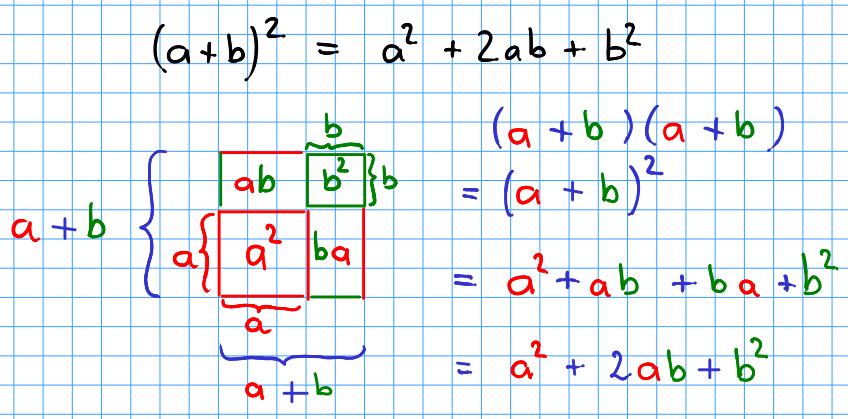
\includegraphics[width=12cm]{allg/alg/img/a_plus_b_zum_quadrat.png}}%
}%% END TNT

\begin{beispiel}{}{}

Typische Anwendungen der binomischen Formeln:

$$(x+5)\cdot(x-5)=\LoesungsRaum{x^2 -25}$$
$$(t+1)\cdot(t-1)=\LoesungsRaum{t^2 - 1}$$
$$(x-2)\cdot(x-2)=\LoesungsRaum{x^2 -4x + 4}$$
\end{beispiel}


\newpage

%Mit diesem Wissen lassen sich einige Summen einfacher ausklammern:
%\vspace{4cm}
%\TRAINER{
%  $$49 - x^2 = (7-x)\cdot(7+x)$$
%  $$a^2 -16a + 64 = (a-8)^2$$
%}

\TALS{
\subsection{Pascalsches Dreieck}\index{Pascalsches
  Dreieck}\index{Dreieck!Pascalsches}

Berechnen Sie $(a+b)^4$:

\TNT{4}{$a^4 + 4a^3b + 6a^2b^2 + 4ab^3 + b^4$}%% END TNT

Zeichnen Sie das Pascalsche Dreieck:
\begin{center}
\begin{tabular}{cccccccccccc}\\
  &   &     &     &     & 1   &     &     &     &     &    & \\
  &   &     &     & 1   &     & 1   &     &     &     &    & \\  
  &   &     & 1   &     & 2   &     & 1   &     &     &    & \\
  &   &  1  &     & 3   &     & 3   &     & 1   &     &    & \\
  & 1 &     & ... &     & ... &     & ... &     & ... &    & \\ 
1 &   & ... &     & ... &     & ... &     & ... &     & ...&  
\end{tabular}
%\noTRAINER{\vspace{3cm}}
\end{center}
\newpage
}


\subsection*{Aufgaben}
%% \TALSAadBMTA{16}{22a) b) e)}
%% \TALSAadBMTA{17}{23a) 24a)}
%% \GESOAadBMTA{36ff}{ 19. b) d) h) 20. a) b) c) d) e) 21. a) 23. a)
%% 24. a) 25. b) e) Optional: 27. c)}
\GESO{\olatLinkArbeitsblatt{Binomische Formeln [A1Bi]}{https://olat.bbw.ch/auth/RepositoryEntry/572162163/CourseNode/105796980058302}{1.) und 2.)}}

\TALS{\olatLinkArbeitsblatt{Binomische Formeln [A1Bi]}{https://olat.bbw.ch/auth/RepositoryEntry/572162090/CourseNode/105796978456639}{1.) und 2.)}}

%%\aufgabenFarbe{Aufgabenblatt im OLAT zu Algebra 1: Binomische
%%Formeln. Aufgaben A1Bi: 1) und 2)}

%%
%% 2019 07 04 Ph. G. Freimann
%%
\newpage
\section{Faktorisieren}\index{Faktorisieren}

\theorieTALS{18}{1.3.2}
\theorieGESO{32}{2.2.3}

%%%%%%%%%%%%%%%%%%%%%%%%%%%%%%%%%%%%%%%%%%%%%%%%%%%%%%%%%%%%%%%%%%%%%%%%%%%%%%%%%
\subsection*{Lernziele}

\begin{itemize}
\item ausklammern
 \begin{itemize}
  \item gemeinsame Faktoren ausklammern
  \item Klammerausdrücke ausklammern
   \begin{itemize}
   \item mehrmaliges Ausklammern (Teilsummen)
  \item -1 ausklammern
  \end{itemize}
\end{itemize}
\item Binomische Formeln
\item Zweiklammeransatz
\TRAINER{\item \textit{(Polynomdivision: kein Lernziel)}}
\item Gemischte Anwendungen
\end{itemize}
\newpage


Beim Faktorisieren werden Summen/Differenzen in Faktoren
zerlegt.

\bbwCenterGraphic{11cm}{allg/alg/img/faktorisieren.png}\index{faktorisieren}\index{ausmultiplizieren}

\subsection*{Fernziel und Nutzen des Faktorisierens}
Betrachten wir die beiden folgenden Bruchterme:
 $$\frac{3x(a^2p - pb^2) - 7pa^2 + 7b^2p}{3a^2xy  + 3yb^2x + 6abyx - 7y(a^2 +b^2) - 14ayb }$$
und
$$\frac{p(3x-7)(a+b)(a-b)}{y(3x-7)(a+b)(a+b)}$$

Beide Terme können durch Termumformungen ineinander übergeführt werden. Mit anderen Worten: Die Terme sind identisch. Doch nur dem zweiten können wir auf einen Blick ansehen, dass er durch Kürzen stark vereinfacht werden kann:

$$\frac{p(a-b)}{y(a+b)}$$

%%%%%%%%%%%%%%%%%%%%%%%%%%%%%%%%%%%%%%%%%%%%%%%%%%%%%%%%%%%%%%%%%%%%%%%%%%%%%%%%%%%%%%%%%%%%%%%%%%%%%
\newpage

\subsection{Ausklammern}\index{ausklammern}
Die gängigste Methode des Faktorisierens ist das Ausklammern.

Das \textbf{Ausklammern}\footnote{Ausklammern wird auch «Vorklammern»\index{Vorklammern!Ausklammern} genannt.} ist die einfachste Umkehrung des Ausmultiplizierens.
Dabei werden gemeinsame Faktoren gesucht und vor (bzw. hinter) eine
neu hinzugefügte Klammer geschrieben.

\subsubsection{gemeinsame Faktoren ausklammern}
Suche gemeinsame Faktoren (Variable, Zahlen) in allen Summanden:

\begin{beispiel}{}{}
  $$4a^3 + 2ab -6a^2x$$
  $$=\noTRAINER{\hspace{7em}}\TRAINER{ {\color{green}2a}\cdot{\color{green}(}2a^2+b -3ax{\color{green})}}$$
\end{beispiel}

\begin{beispiel}{Woher kommt die Eins?}{}

$$4a^3 + 2a^2$$
$$=\noTRAINER{\hspace{7em}}\TRAINER{2a^2(2a + 1)}$$
Wenn wir die Faktoren zurück ausmultiplizieren, sehen wir, dass die
Eins (1) nicht fehlen darf. \textbf{Tipp}: Zur Probe immer zurück ausmultiplizieren.
\end{beispiel}

\newcommand{\olatAB}[2]{\subsection*{Aufgaben}
\aufgabenFarbe{OLAT #1. Aufg. #2}
\platzFuerBerechnungenBisEndeSeite{}}

\olatAB{Algebra I Faktorisieren Aufgabenblatt A1F}{1}

%%\GESO{\aufgabenFarbe{S. 38: Aufg. 37. 38. a) e) }}
\newpage


\subsubsection{Minus Eins ausklammern I}

\textbf{Vertauschte Differenz}\\

$$8-a = \LoesungsRaumLang{\mathbf{(-1)\cdot{}} (-8 + a) = -(a-8)}$$

Anwendung:
$$\frac{a-3}{3-a} = \LoesungsRaumLang{\frac{(-1)\cdot{}(-a+3)}{3-a}} = \LoesungsRaumLang{\frac{(-1)\cdot{}(3-a)}{3-a}} = \frac{-1}1 = -1$$

Aus jeder Summe (bzw. Differenz)
kann minus Eins $(-1)$ ausgeklammert werden, indem alle Vorzeichen der
Summanden umgedreht werden:

$$ -4 + x - 5\cdot(a-b) +c  =\LoesungsRaumLang{ {\color{ForestGreen} (-1)}\cdot{} ({\color{ForestGreen}+}4 {\color{ForestGreen}-}x {\color{ForestGreen}+}
5\cdot{(a{\color{red}-}b)} {\color{ForestGreen}-}c)}$$

Achtung oben: Das Vorzeichen bei $a-b$ ändert sich nicht, denn dies
ist nicht ein Vorzeichen der globalen Summanden!

%%\subsection{Aufgaben}
%%\GESOAadB{39}{39. h) i)}
%%\GESOAadB{39}{40. a)}

\olatAB{Algebra I Faktorisieren Aufgabenblatt A1F}{2}

\newpage


\subsubsection{Identische Klammerausdrücke}\index{Klammerausdruck ausklammern}
Anstelle einfacher Monome können auch ganze Klammerausdrücke
ausgeklammert werden:
$$7x{\color{green}(3+b)} + 5z{\color{green}(b+3)}$$
$$=(7x+5z){\color{green}(3+b)}$$

Tipp: Geben Sie dem Klammerausdruck einen Namen\footnote{Dieser
chinesische Rechentrick löst manches {\color{green}A} bzw. {\color{green}Aha}-Erlebnis aus!}: ${\color{green}A} = {\color{green}(3+b)}$, dann liest sich der
Term wie folgt:
$$7x{\color{green}(3+b)} + 5z{\color{green}(b+3)} = 7x\cdot{\color{green}A}
+ 5z\cdot{\color{green}A} {\stackrel{\textrm{a.}}{=}}
(7x+5z)\cdot{\color{green}A} = (7x+5z){\color{green}(3+b)}$$

\begin{beispiel}{}{}
$$6b(5+x) - x- 5$$
\TNT{5.2}{
$$6b(5+x) -(x+5)$$
$$6b(5+x) -1(x+5)$$
$$6b(x+5) -1(x+5)$$
$$(x+5) (6b-1)$$
}

\end{beispiel}

\olatAB{Algebra I Faktorisieren Aufgabenblatt A1F}{3}


\newpage



\subsubsection{Minus Eins ausklammern II}\index{Minus Eins ausklammern}
Unterscheiden sich Teilklammern nur durch Vorzeichen, so bietet es
sich an, Minus Eins (-1) auszuklammern, um identische Klammerausdrücke
zu erhalten:
$$7x{\color{green}(b-3)} + 5z{\color{green}(3-b)}$$%%

\TRAINER{%%

$7x{\color{green}(b-3)} - 5z{\color{green}(-3+b)}$
\vspace{10mm}
}%%

\TRAINER{%%

$7x{\color{green}(b-3)} - 5z{\color{green}(b-3)}$
\vspace{10mm}
}%%


\noTRAINER{\mmPapier{3.6}}


\olatAB{Algebra I Faktorisieren Aufgabenblatt A1F}{4}

%%\TALSAadB{18}{29. b), 30. a) c) d) g), 31. a) c) f), i) und 32. b) f)}
%%\GESOAadB{39}{41. a) e) d) 42. b) c) 43. b) c) 44. b) e) }
\newpage



\subsubsection{Mehrmaliges Ausklammern:}\index{ausklammern!mehrmaliges}
 Um identische Klammerausdrücke zu finden, bietet sich die Methode des mehrmaligen Ausklammerns an.
 Dabei wird die Summe (bzw. Differenz) in gleiche Anzahl \textbf{Teilsummen}\index{Teilsummen} aufgeteilt und Stückweise ausgeklammert.
 Im folgenden Beispiel werden die beiden ersten Summanden und die beiden letzten «Summanden» zunächst unabhängig voneinander betrachtet.

$$3mk+6nk-5m-10n $$
$$= 3k{\color{green}(m+2n)}-5{\color{green}(m+2n)} $$
$$= (3k-5){\color{green}(m+2n)}$$


\begin{beispiel}{}{}
  $$5a-30+ax-6x = ...$$
  Wie gehen wir vor? Beispiel: Aus den ersten beiden Summanden 5 und
  aus den beiden hinteren Summanden $x$ ausklammern:

\TNT{2.4}{$$... = 5\cdot(a-6) + x\cdot(a-6) = ...$$}

  Nun aus beiden Summanden den Term ......... \TRAINER{$(a-6)$}
  ausklammern:

\TNT{2.4}{$$... = (5+x)\cdot(a-6)$$}
\end{beispiel}

\olatAB{Algebra I Faktorisieren Aufgabenblatt A1F}{5}

\newpage


\subsection{Binomische Formeln}\index{Faktorisieren!mit binomischen Formeln}%%
\index{Binomische Formeln!zum Ausklammern}

\GESO{S. Kap. 2.2.3 S. 32 \cite{marthaler21}}%%
\TALS{S. 18 Kap. 1.3.2 \cite{frommenwiler17alg}}


Zerlegen wir die folgenden Terme in einzelne Faktoren:
$$ a^2 - 16 = \LoesungsRaum{(a+4)(a-4)} $$

$$x^2 -18x + 81 = \LoesungsRaum{(x-9)(x-9)}$$

$$64y^2 - 49z^6 = \LoesungsRaum{(8y+7z^3)(8y-7z^3)}$$

$$c^4 - 1 = \LoesungsRaum{\mathbf{(c+1)(c-1)}(c^2+1)}$$

\TALS{$$ b^3 - 3b^2a + 3ba^2 - a^3 = \LoesungsRaum{(b-a)^3}$$}

\olatAB{Algebra I Faktorisieren Aufgabenblatt A1F}{6}

%%\TALSAadB{19}{33. a) b) c) h) l) und 34. a)}
%%\GESOAadB{39ff}{41. c), 45. a) b) c) d) e), 46. a) c) e) g) und  47. a) b) e) c)}
\newpage



\subsection{Zweiklammeransatz}\index{Zweiklammeransatz}
Beispiel $$a^2-4a-5$$
$$=(a-\Box{})(a+\Box{}) = (a-5)(a+1)$$

\GESO{\noTRAINER{\mmPapier{5.2}}\TRAINER{Optional: Taschenrechner poly-solv, danach Vorzeichen
drehen!

Beispiel $x^2 - 2x -48$;

lösen wir mit $a=1$, $b=-2$ und
$c=-48$. Taschenrechner Lösungen 8 und -6. Somit lautet die
faktorisierte Form (nach dem Tauschen der Vorzeichen):
$$x^2-2x-48 = (x-8)(x+6)$$}}%% END GESO

\begin{rezept}{Zweiklammeransatz}{}
Gegeben ist eine Summe mit drei Summanden:
$$x^2 \pm A\cdot{}x \pm B$$

1. Zwei Klammern bereitstellen (= Zweiklammer-Ansatz):
$$(x \,\,\,\,\,\,\, \Box)\cdot{}(x \,\,\,\,\,\,\, \Box)$$
2. Vorzeichen bestimmen:
\leserluft{}

  \begin{tabular}{|c@{$\Longrightarrow$}c|}\hline
   $x^2 + A\cdot{} x + B$ & $(x + \Box)\cdot{}(x + \Box)$\\\hline
   $x^2 - A\cdot{} x + B$ & $(x - \Box)\cdot{}(x - \Box)$\\\hline
   $x^2 ... A\cdot{} x \mathbf{-} B$ & $(x + \Box)\cdot{}(x - \Box)$\\\hline
   \end{tabular} 

\leserluft{}

3. $B$ in Faktoren zerlegen und versuchen $A$ als Summe dieser Faktoren zu schreiben.
\end{rezept}
\newpage
\begin{beispiel}{Zweiklammeransatz}{}
Beispiel
$$x^2 - 4x - 12$$
\TNT{8}{$$\Longrightarrow B=12 = 1\cdot{}12 = 2\cdot{}6 = 3\cdot{}4$$
$$\Longrightarrow x^2-4x-12 = (x-6)\cdot{}(x+2)$$}%% END TNT
\end{beispiel}


\olatAB{Algebra I Faktorisieren Aufgabenblatt A1F}{7}


%%\TALSAadB{19}{35. a) b) d) k)}
%%\GESOAadB{40}{48. a) d) g) h) i) 49. a) b) c) d)}

\newpage


%\noTRAINER{\blankpage{}}
\subsection{Gemischte Anwendung (Optional)}
Im folgenden Beispiel kommen alle obigen Vorgehensweisen als
Teilschritte vor:

\begin{center}{\fbox{$ a^2px^2 - 9pa^2 + 36pa -4xpxa -5px^2 + 45p$}}\end{center}

%%\begin{center}{\fbox{$$ a^2px^2 - 9pa^2 + 36pa -4xpxa -5px^2 + 45p$$}}\end{center}

1. Gemeinsame Faktoren (hier $p$) ausklammern:
$$p[a^2x^2 - 9a^2 + 36a -4x^2a -5x^2 + 45]$$
2. Teilsummen ausklammern, um gemeinsame Klammerausdrücke zu finden\footnote{
Analog könnte auch wie folgt ausgeklammert werden:
$$p[{\color{green}a^2x^2 -9a^2} {\color{red}+ 36a -4x^2a} {\color{blue}- 5x^2 + 45}]$$
$$p[{\color{green}a^2}(x^2 - 9) + {\color{red}4a}(9 - x^2) + {\color{blue}5}(-x^2 + 9)]$$
}
:
$$p[{\color{green}a^2x^2 } {\color{red}\, -\, 9a^2} {\color{red}\, +\, 36a} {\color{green}\, -\, 4x^2a} {\color{green} {\color{green}\,-\,5x^2} } + {\color{red}45}]$$
$$p[{\color{green}x^2} (a^2 -4a -5) + {\color{red}9}(-a^2 + 4a +5)]$$

3. Minus Eins (-1) ausklammern:
$$p[x^2 (a^2 -4a -5) {\color{green}-} 9({\color{green}+}a^2 {\color{green}-} 4a {\color{green}-} 5)]$$
4. Klammerausdrücke ausklammern:
$$p[x^2 {\color{blue}(a^2 -4a -5)} - 9{\color{blue}(+a^2 - 4a - 5)}]$$
$$p[(x^2-9) {\color{blue}(a^2 -4a -5)}]$$
$$p(x^2-9) (a^2 -4a -5)$$
5. Binomische Formel:
$$p{\color{green}(x^2-9)}(a^2 -4a -5)$$
$$p{\color{green}(x+3)(x-3)}(a^2 -4a -5)$$

6. Zweiklammeransatz:
$$p(x+3)(x-3) (a-\Box{})(a+\Box{})$$

Welche Zahlen ergeben multipliziert $-5$ und addiert $-4$?
$$p(x+3)(x-3)(a+5)(a-1) ???$$
\begin{center}{\fbox{$p(x+3)(x-3)(a-5)(a+1)$}}\end{center}



\olatAB{Algebra I Faktorisieren Aufgabenblatt A1F}{8}
%%\TALSAadB{19ff}{41. c), 43. b), 44. }%% end TALS
%%\GESOAadB{40}{50. a) b) d) und 51. a) b) c)}

\newpage

%%
%% 2019 07 04 Ph. G. Freimann
%%
\newpage
\section{Bruchterme}\label{bruchterme}\index{Bruchterme}
\sectuntertitel{Wer sich mit einem Mathematiker anlegt, muss mit einem
  Bruch rechnen.}

%%%%%%%%%%%%%%%%%%%%%%%%%%%%%%%%%%%%%%%%%%%%%%%%%%%%%%%%%%%%%%%%%%%%%%%%%%%%%%%%%
\subsection*{Lernziele}

\begin{itemize}
	\item Begriffe: Dividend (Zähler)\index{Dividend} :
  Divisor/index{Divisor} (Nenner) = Quotient\index{Quotient} (Bruch)
  \item Kürzen (und erweitern)
	\item Gleichnamig machen\index{gleichnamig}, Hauptnenner\index{Hauptnenner} (kgV\index{kgV}\GESO{\cite{marthaler21alg} Seite 43})
	\item Brüche addieren/subtrahieren
  \item multiplizieren
	\item Doppelbrüche (Brüche dividieren) S. 45 \cite{marthaler21alg}
\end{itemize}


\TadBMTA{41}{3}
\newpage

\subsection{Erweitern und Kürzen}\index{Erweitern}\index{Kürzen}
\TadBMTA{42}{3.2}

Jeder Bruch kann ohne ändern seines Wertes erweitert bzw. gekürzt
werden:

\subsubsection{Kürzen}
$$\frac{1030}{500} = \LoesungsRaumLang{\frac{1030 : 10}{500:10} =\frac{103}{50}}$$
\TRAINER{nicht einfach die beiden Nullen streichen!}


\subsubsection{Erweitern}
$$\frac{4.6}{9.45} = \LoesungsRaumLang{\frac{4.6 \cdot{}100}{9.45\cdot{}100} =
\frac{460}{945}}$$
\newpage


\begin{beispiel}{}{}
$$\frac{ax^2 - a}{(a^2+1)(ax+a)} = \noTRAINER{\hspace{10cm}}\TRAINER{\frac{a\cdot{}(x^2-1)}{(a^2+1)\cdot{}a\cdot{}(x+1)}=\frac{a\cdot{}(x+1)\cdot{}(x-1)}{(a^2+1)\cdot{}a\cdot{}(x+1)}=\frac{x-1}{a^2+1}} $$
\end{beispiel}

\begin{beispiel}{Mit -1 erweitern}{}

$$\frac{a-b}{b-a} = \frac{\TRAINER{(-1)}\noTRAINER{\hspace{20mm}}\cdot(a-b)}{\TRAINER{(-1)}\noTRAINER{\hspace{20mm}}\cdot(b-a)}
= \frac{\TRAINER{(-1)\cdot(a-b)}}{\TRAINER{+a-b}\noTRAINER{\hspace{30mm}}} = \LoesungsRaum{-1}$$
\end{beispiel}


\begin{rezept}{}{}

\begin{center}Bei Brüchen, das steht hier gedruckt:\\
\textbf{«Wir kürzen nur aus dem Produkt.»}\\

Ich habe deshalb mir geschworen.\\
Ich kürz' ab jetzt nur noch Faktoren.\\

Steht jedoch was zum Addieren,\noTRAINER{\vspace{5mm}}\\
muss ich erst \noTRAINER{\hspace{5cm}}\TRAINER{\textbf{faktorisieren}}!\\
\end{center}
\end{rezept}


\subsection*{Aufgaben}
\AadBMTA{48ff}{5. d), 6. a), 7. a), 8. a)\TALS{ c)}, 9. c) h), 10. b),
11. a) c) d) e) f), \GESO{(Optional 12.,)}\TALS{12.,} 13. a)}%

\AadBMTA{48ff}{2. d)}%

\newpage

\subsection{Definitionsmenge}\index{Definitionsmenge!Bruchterme}\index{Definitionsmenge@Definitionsbereich}

\begin{definition}{Definitionsmenge}{}
Die Menge aller Zahlen, die für die Variable in einen Term (\zB einen
Bruch) eingesetzt werden darf, nennen wir
die \textbf{Definitionsmenge} $\mathbb{D}$ oder den \textbf{Definitionsbereich}.
\end{definition}

%%\renewcommand{\arraystretch}3
\begin{bbwFillInTabular}{c|c|l}%%
Bruch                  & Was darf nicht eingesetzt werden? & $\mathbb{D}$ Definitionsmenge \\\hline
$\frac1x$              & \TRAINER{0}                       & \TRAINER{$\mathbb{D}=\mathbb{R}\backslash\{0\}$}\\\hline  
$\frac1{2-x}$          & \TRAINER{2}                       & \TRAINER{$\mathbb{D}=\mathbb{R}\backslash\{2\}$}\\\hline
$\frac{x}{(x-5)(x+3)}$ & \TRAINER{-3; 5}                   & \TRAINER{$\mathbb{D}=\mathbb{R}\backslash\{-3; 5\}$}\\\hline
$\frac{5}{5x^2-5x-60}$ & \TRAINER{-3; 4}                   & \TRAINER{$\mathbb{D}=\mathbb{R}\backslash\{-3; 4\}$}\\\hline
\end{bbwFillInTabular}


\TNT{4}{$$5x^2 - 5x - 60 $$   $$= 5(x^2-x-12) $$   $$= 5(x-4)(x+3)$$}

\subsection*{Aufgaben}

\AadBMTA{48ff}{3. c) d)}%



\newpage
\subsection{Rechnen mit Bruchtermen}
\TadBMTA{43ff}{3.3 und 3.4}
%%\TALSTadBMTA{43}{3.3} \TALS{und} \TadBMTA{44}{3.4}

\subsubsection{Addition und Subtraktion von Bruchtermen}

Vorzeigeaufgabe:

$$\frac{6t}{3r} + 2r - \frac{2ar+2ta}{ra}$$

\TNTeop{
Einzelbrüche faktorisieren
$$\frac{2\cdot{}3\cdot{}t}{3\cdot{}r}  + 2r - \frac{2a(r+t)}{r\cdot{}a}$$

Kürzen
$$\frac{2t}r + \frac{2r}1 -  \frac{2(r+t)}{r}$$

Erweitern auf Hauptnenner (HN = $r$) = gleichnamig machen
$$\frac{2t}r + \frac{2r^2}r -  \frac{2(r+t)}{r}$$

Selber Bruchstrich
$$\frac{2t + 2r^2 - 2(r+t)}r$$

Zähler ausrechnen / ausmultiplizieren
$$\frac{2t + 2r^2 -2r -2t}r$$
Zähler Zusammenfassen und vereinfachen
$$\frac{2r^2 - 2r}r$$

Zähler faktorisieren
$$\frac{2r(r-1)}r$$

Kürzen


$$\frac{2(r-1)}{1} = 2(r-1)$$

Welche Rezepte leiten wir daraus ab?
}

%%%%%%%%%%%%%%%%%%%%%%%%%%%%%%%%%%%%%%%%%%%%%%%%%%%%%%%%%%%%%%%%%%%%%%%%%%555

\begin{rezept}{Brüche addieren/subtrahieren}{}\label{bruchtermeRezept}
\begin{enumerate}
	\item Einzelbrüche faktorisieren
  \item Definitonsmenge $\mathbb{D}$ bestimmen
	\item Einzelbrüche kürzen
	\item gemeinsamen Nenner finden (Hauptnenner, von Vorteil
	kgV). \textbf{Achtung}: Beim \textbf{Multiplizieren nicht}
	gleichnamig machen. Beim \textbf{Dividieren} im rechten Bruch Zähler
	und Nenner tauschen: Die Division wird zur Multiplikation.
	\item Brüche auf Hauptnenner erweitern
	\item Alle Zähler auf den selben Bruchstrich schreiben (Vorzeichen beachten, Klammern setzen)
	\item Im Zähler ausmultiplizieren
	\item Zähler zusammenfassen und vereinfachen
	\item Zähler faktorisieren
	\item kürzen
\end{enumerate}
\end{rezept}


\begin{gesetz}{}{}
Merksatz: Nur gleichnamige Brüche dürfen addiert (bzw. subtrahiert)
werden.
\end{gesetz}



\subsection*{Aufgaben}

\AadBMTA{49ff}{20. e), 21. b) f), 22. d) f), 23. a) b) g) h), 24. a), 25. a) b)\TALS{ d), } 26.\GESO{*} c) d)}%

\newpage

\subsubsection{Rechentrick (optional)}
Bei teilerfremden Brüchen bietet sich folgender Rechentrick an:

\begin{gesetz}{Addieren von Brüchen}{}
$$\frac{a}{b} + \frac{x}{y} = \frac{ay + bx}{by}$$
\end{gesetz}

\newcommand{\miniPlatz}[1]{\noTRAINER{\,\,\,\,\,\,}\TRAINER{#1}}

Herleitung
$$\frac{a}{b} + \frac{x}{y} = %% \frac{a}{b}\cdot\frac{y}{y} +  \frac{x}{y}\cdot\frac{b}{b} =
%%\frac{a\cdot y}{b\cdot y} + \frac{x\cdot b}{y \cdot b}
\frac{a\miniPlatz{\cdot{}y}}{b\miniPlatz{\cdot{}y}} + \frac{x\miniPlatz{\cdot{}b}}{y\miniPlatz{\cdot{}b}} = \LoesungsRaum{\frac{ay + bx}{by}}$$


\begin{beispiel}{}{}
$$\frac{a+1}{-a} + \frac{a}{a-1} = \noTRAINER{\hspace{2cm}}\LoesungsRaumLang{ \frac{a^2 - 1 - a^2}{-a(a-1)} = \frac{1}{a(a-1)}}$$
\end{beispiel}

\TNTeop{}%% end TNTeop
\newpage


\subsubsection{Multiplikation von Bruchtermen}

\begin{gesetz}{}{}
$$\frac{a}{b}\cdot\frac{x}{y} = \frac{a\cdot x}{b\cdot y} = \frac{ax}{by}$$
\end{gesetz}

\begin{beispiel}{«von» heißt «mal»}{}
Was sind $\frac34$ von 600?
\TNT{3.2}{
600 / 4 = 150 und 150 * 3 = 450, das ist das selbe wie
$\frac34\cdot{}600 = 450$
}
\begin{center}\fbox{Von = Mal\footnote{Bei Bruchtermen, Prozentzahlen und
Häufigkeitsfaktoren kann man das «von» als Multiplikation
auffassen. $20\% \text{ von } 67 = 0.2 \cdot{} 67$; aber auch
$\frac{1}{3} \text{ von } 5
= \frac{1}{3}\cdot{5} = \frac{5}{3}$. Dies stimmt jedoch nur bei
Brüchen, Prozentzahlen und Häufigkeitsfaktoren: Bei Anzahlen,
metrischen Werten und dergleichen ist dann das «von» durch eine
Division zu ersetzen und wir erhalten dann den Bruch
(bzw. Prozentsatz). Beispiel: Drei von fünf Kindern heißt $\frac{3}{5}
= 60\% = 0.6$.}}\end{center}

\end{beispiel}


$$\frac34 \text{ von } \frac23 = \frac34\cdot\frac23
=  \frac23\cdot\frac34 = \frac23 \text{ von } \frac34$$

\TRAINER{\bbwCenterGraphic{8cm}{allg/alg/img/UhrDreiViertel.png}}
\noTRAINER{\bbwCenterGraphic{8cm}{allg/alg/img/UhrDreiViertelLeer.png}}

\subsubsection{Division von Bruchtermen}
\begin{gesetz}{}{}
$$\frac{a}{b} : \frac{x}{y}=\frac{a}{b}\cdot\frac{y}{x} = \frac{a\cdot y}{b\cdot x} = \frac{ay}{bx}$$
\end{gesetz}

Begründung — mit Kehrwert erweitern:

$$5 : \frac{3}{4} = \LoesungsRaumLang{
\frac{5}{\left(\frac{3}{4}\right)} =
\frac{5\cdot{}\frac43}{\frac34\cdot{}\frac43} =
\frac{5\cdot{}\frac43}{1} = 5 \cdot{} \frac43}$$
\newpage

\subsubsection{Doppelbrüche}\index{Doppelbruch}

%%\TALS{S. Buch \cite{frommenwiler17alg} S. 25 Kap. 1.4.4 Dividieren.}
%%\GESO{S. Buch \cite{marthaler21alg} S. 44 Kap. 3.4 Brüche multiplizieren und dividieren}

\TadBMTA{44/45}{3.4}

\begin{definition}{Doppelbruch}{definition_doppelbruch}\index{Doppelbruch}
  \textbf{Doppelbrüche} sind lediglich eine andere Schreibweise für die
  Division zweier Brüche:\\

  \begin{center}
  \fbox{\huge{$\frac{\frac{a}{b}}{\frac{c}{d}} = \frac{a}{b} :
      \frac{c}{d}$}}
  \end{center}
\end{definition}

\begin{gesetz}{Doppelbruch}{gesetz_doppelbruch}\index{Doppelbruch}
  Brüche werden dividiert, indem man mit dem Kehrwert des Divisors multipliziert:\\

  \begin{center}
  \fbox{\huge{$\frac{\frac{a}{b}}{\frac{c}{d}} = \frac{a}{b} :
      \frac{c}{d} = \frac{a}{b} \cdot\frac{d}{c} = \frac{ad}{bc}$}}
  \end{center}
\end{gesetz}

\begin{beispiel}{}{}
$$\frac{\frac{x+1}{x^2-1}}{\frac{x^2+2x+1}{-2-2x}}$$
\end{beispiel}

\TNTeop{
  $= \frac{x+1}{x^2-1}      :     \frac{x^2+2x+1}{-2-2x}$
  $= \frac{x+1}{(x-1)(x+1)} :     \frac{(x+1)(x+1)}{-2(1+x)}$
  $= \frac{x+1}{(x-1)(x+1)} \cdot \frac{(-2)(1+x)}{(x+1)(x+1)}$
  $= \frac{ -2}{(x-1)(x+1)}$
}




\newpage
\subsection*{Aufgaben}
\GESOAadBMTA{51ff}{27. 28. b) f) 29. d) e) 30. d) e) 31. b) 32. a) 33. a) 34. a) 35. b) 36. d) 37. a) 38. d)}%
\TALSAadBMTA{51ff}{27. 28. b) f) 29. d) e) 30. d) e) 31. b) 32. a)
33. a) f) 34. a) 35. b) 36. d) 37. a) 38. d), 39. c)}%
%


\GESO{\olatLinkArbeitsblatt{Bruchterme
vereinfachen
(Maturaaufgaben)}{https://olat.bbw.ch/auth/RepositoryEntry/572162163/CourseNode/106261572709001}{Ab
Jahr 2017}}%% END olatLinkArbeitsblatt

\olatLinkGESOKompendium{1.3}{8}{13}

\newpage


%%
%% 2019 11 14 ph. freimann
%%

\newpage
\subsection{Minus Eins (optional)}\index{Minus Eins}\index{$-1$}

\subsubsection*{Was wir mit der $(-1)$ tun dürfen}

\begin{tabular}{p{5cm}|rcl}
  \hline\\
  Notation          & $(-1)\cdot(...)$                &$=$& $-(...)$                      \\
  \\
  \hline\\
  Ausmultiplizieren & $(-1)\cdot(7x-4y+3-2b)$              &$=$& $-7x + 4y -3 + 2b$            \\
                    & $-(-4a + 3v -(x+2))$            &$=$& $-(-4a +3v -x-2)$             \\
                    &                                 &$=$& $+4a -3v +x+2$                \\
  \\
  \hline\\
  Ausklammern       & $-7x +4y -3 +2b$                &$=$& $(-1)\cdot (+7x -4y + 3 -2b)$ \\
                    & $4a -3v + x +2$                 &$=$& $-(-4a + 3v -x -2)$           \\
  \\
  \hline\\
  Erweitern         & $\frac{-7x+3b -8}{3x - 4y -16}$ &$=$& $\frac{{\color{ForestGreen}(-1)}\cdot(-7x+3b -8)}{{\color{ForestGreen}(-1)}\cdot(3x - 4y -16)}$\\
                    & $\frac{a-b}{b-a}$               &$=$& $\frac{{\color{ForestGreen}(-1)}\cdot(a-b)}{{\color{ForestGreen}(-1)}\cdot(b-a)}$\\
  \\
  \hline\\                      
  Erweitern und Ausmultiplizieren  & $\frac{-7x+3b -8}{3x - 4y -16}$ &$=$& $\frac{(-1)\cdot(-7x+3b -8)}{(-1)\cdot(3x - 4y -16)}$\\
                    &                                 &$=$& $\frac{7x-3b+8}{-3x+4y+16}$\\
  \\
  \hline\\                    
  Gemischtes
  Beispiel          & $\frac{a-b}{b-a}$               &$=$& $\frac{a-b}{(-1)\cdot(-b+a)}$ \TRAINER{-1 auskl.}\\
                    &                                 &$=$& $\frac{(a-b)}{(-1)(a-b)}$ \TRAINER{kommutativ}\\
                    &                                 &$=$& $\frac{1}{(-1)}$ \TRAINER{kürzen}\\
                    &                                 &$=$& $\frac{(-1)\cdot 1}{(-1)\cdot(-1)}$\TRAINER{(-1) erw.}\\
                    &                                 &$=$& $\frac{(-1)\cdot 1}{1}$ \TRAINER{(-1)(-1)=(+1)}\\
                    &                                 &$=$& $-1$ \TRAINER{kürzen}\\
\end{tabular}

\paragraph{Gleichungen} Bei Gleichungen dürfen beide Seiten des Gleichheitszeichens mit (-1) multipliziert werden (sofern man wirklich \textbf{beide} Seiten multipliziert). 

\newpage
\subsubsection*{Was wir mit der Minus Eins nicht tun!}
Wir multiplizieren nicht einfach einen Term mit \textit{Minus Eins}.
Gegenbeispiel:

Konto Hr. Ph. Freimann Stand 1. Jan. 2025: CHF {\color{ForestGreen}10\,377.--}.

Multiplikation am 2. Jan. 2019 mit $(-1)$.

Konto Hr. Ph. Freimann Stand 3. Jan. 2025: CHF {\color{red} -10\,377.--}.
\newpage


%%\TALSAadBFWA{21ff}{45. a) c) 46. c) d) 47. a) b) c) e) 48. a) 49. a)
%%       S. 23ff: 52. b) 53. b) 54. Mit TR: a) b) c) Von Hand: 57. b) c)
%%       d) TR: 58. a) b) Hand: 59. b) c) TR: 60. b) c) d) }
\newpage

\newpage
